\documentclass[paper=a4, fontsize=12pt]{article} % A4 paper and 11pt font size
\usepackage[T1]{fontenc} % Use 8-bit encoding that has 256 glyphs
\usepackage[english]{babel} % English language/hyphenation
\usepackage{amsmath,amsfonts,amsthm} % Math packages
\usepackage{a4wide}
\usepackage{float}
\usepackage{longtable}
\usepackage{hyperref}
\usepackage{listings}
\usepackage{makecell}
\usepackage{graphicx}
\usepackage[table]{xcolor}
\usepackage[numbered, framed]{mcode}  % To load matlab code
\lstset{deletestring=[b]{"}}

\usepackage{fancyhdr} % Custom headers and footers
\pagestyle{fancyplain} % Makes all pages in the document conform to the custom headers and footers
\setlength\parindent{0pt}
\fancyhead[L]{SF3565, Project 4, December 2016}
\fancyhead[R]{H{\"a}ggmark, Karlsson} % Empty left footer
\fancyfoot[C]{Program construction in C++ for Scientific Computing} % Empty center footer
\fancyfoot[R]{\thepage} % Page numbering for right footer

\title{Program construction in C++ for Scientific Computing \\ Teacher: Michael Hanke}

\author{Ilian H{\"a}ggmark \\ mail \href{mailto:ilianh@kth.se}{ilianh@kth.se}
  \and Andreas Karlsson \\ mail \href{mailto:andreas.a.karlsson@ki.se}{andreas.a.karlsson@ki.se} }
\date{\normalsize\today} % Today's date or a custom date

\begin{document}

\maketitle % Print the title

\section*{Project 4}
\subsection*{Task 1 - Redesign Domain class}


\subsection*{Task 2 - GFkt class}

The discrete differential operator $\frac{\partial}{\partial x}$  can be approximated as simply $u(x+1,y)-u(x-1,y)$ and analogously for $y$. The second order derivative can be approximated with $u(x+1,y)-2 \cdot u(x,y) + u(x-1,y)$ for the $x$-direction. The Laplacian can be expressed as 

$$ 
 \begin{bmatrix}
  0 & 1 &  0 \\
  1 & -4 &  1 \\
  0 & 1 &  0
 \end{bmatrix}
 $$
 
 The code below shows these approximate derivatives in \textsc{Matlab}:

\begin{lstlisting}
% Approximate partial derivatives

x = -30:0.1:30;
y = -5:0.1:5;

ux = sin((x/10).^2).*cos(x/10); % x-comp of u(x,y)
[X,Y] = meshgrid(ux,y);
u = X+Y;

Dx = zeros(size(u));    % first partial derivative in x
Dy = zeros(size(u));    % first partial derivative in y
L = zeros(size(u));     % laplacian

for i = 2:(length(x)-1)
    for j = 2:(length(y)-1)
        Dx(j,i) = u(j,i+1)-u(j,i-1);
        Dy(j,i) = u(j+1,i)-u(j-1,i);
        L(j,i) = -4*u(j,i)+u(j-1,i)+u(j+1,i)+u(j,i-1)+u(j,i+1);
    end
end
\end{lstlisting}

\subsection*{Task 3 - Discrete differential operators}

The function $u(x,y)$ and its derivatives are shown below

\begin{align*}
u(x,y) &= \sin\left(\left(\frac{x}{10}\right) ^2\right ) \cos(x/10)+y \\
\frac{\partial}{\partial x} u(x,y) &= \frac{2}{100}x\cos\left(\left(\frac{x}{10}\right) ^2\right )\cos\left(\frac{x}{10}\right )- \frac{1}{10}\sin\left(\left(\frac{x}{10}\right) ^2\right )\sin\left (\frac{x}{10}\right )\\
\frac{\partial}{\partial y} u(x,y) &= \frac{\partial}{\partial y}y = 1   \\
\frac{\partial^2}{\partial x^2} u(x,y) &= \frac{2}{100}\cos\left(\left(\frac{x}{10}\right) ^2\right )\cos\left(\frac{x}{10}\right ) - \left ( \frac{2}{100}x\right )^2 \sin \left(\left(\frac{x}{10}\right) ^2\right )\cos\left(\frac{x}{10}\right ) \\
 &- \frac{2}{100}\frac{1}{10}\cos\left(\left(\frac{x}{10}\right) ^2\right )\sin\left(\frac{x}{10}\right ) - \frac{1}{10}\frac{2}{100}x \cos\left(\left(\frac{x}{10}\right) ^2\right )\sin\left (\frac{x}{10}\right )\\
 & - \frac{1}{100}\sin\left(\left(\frac{x}{10}\right) ^2\right )\cos\left (\frac{x}{10}\right )\\
\frac{\partial^2}{\partial y^2} u(x,y) &= 0 \\
\Delta u(x,y) &= \frac{\partial^2}{\partial x^2} u(x,y) + \frac{\partial^2}{\partial y^2} u(x,y) =  \frac{\partial^2}{\partial x^2} u(x,y)
\end{align*}


The code below plot the algebraic expressions in \textsc{Matlab}

\begin{lstlisting}
% Algebraic expressions of first and second partial derivatives in x

x = -50:0.1:50;

figID = figure(101);                             % open figure

ux = sin((x./10).^2).*cos(x./10);                % x-component of u(x,y)

dxu = 2/100.*x.*cos((x./10).^2).*cos(x./10) ...  % first parital derivative
      - 1/10*sin((x./10).^2).*cos(x./10);

dxxu = 2/100*cos((x./10).^2).*cos(x./10) ...     % second partial derivative
       - (2/100.*x).^2.*sin((x./10).^2).*cos(x./10) ...
       - 1/250*cos((x./10).^2).*sin(x./10) ...
       - 1/100*sin((x./10).^2).*cos(x./10);
       
subplot(1,3,1); plot(x,ux);
subplot(1,3,2); plot(x,dxu);                     % plot result in subplot
subplot(1,3,3); plot(x,dxxu);

\end{lstlisting}


\begin{figure}[H]
  \centering
  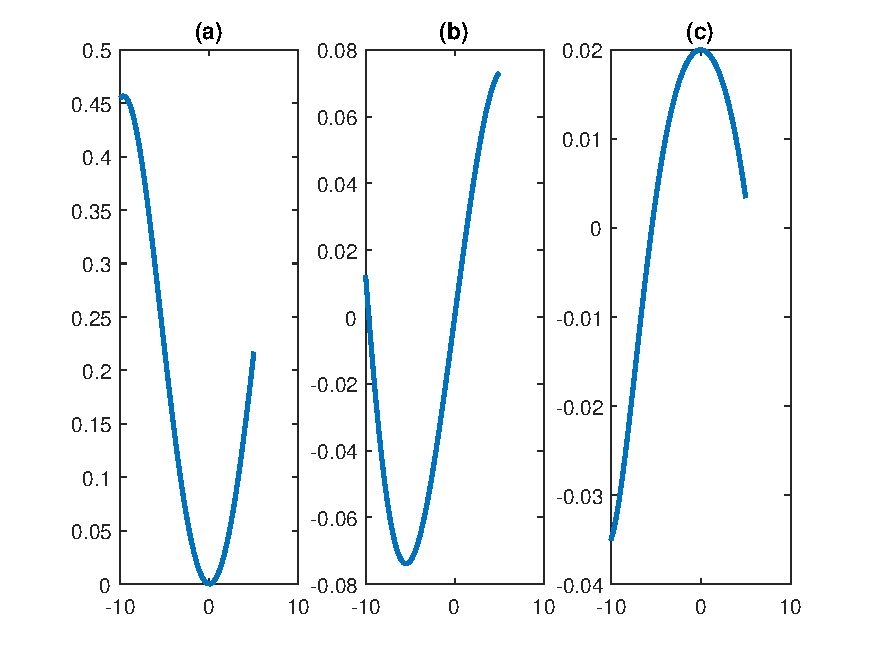
\includegraphics[width=\textwidth]{algebraicDeriv.pdf}
  \caption{\small (a) x-component of $u(x,y)$. (b) First partial derivative of $u(x,y)$ in x. (c) Second partial derivative of $u(x,y)$ in x.\label{fig:stretched}}
\end{figure}



\end{document}
